\documentclass[xcolor=pdflatex,dvipsnames,table]{beamer}
\usepackage{epsfig,graphicx}
\usepackage{palatino}
\usepackage{fancybox}
\usepackage{relsize}
\usepackage[procnames]{listings}
\usepackage{hyperref}
\usepackage{qtree} % needed?
\usepackage{booktabs}
\usepackage{dirtree}
\usepackage[normalem]{ulem}


% fatter TT font
\renewcommand*\ttdefault{txtt}
% another TT, suggested by Alex
% \usepackage{inconsolata}
% \usepackage[T1]{fontenc} % needed as well?


\newcommand{\scale}{0.7}

\newcommand{\todo}[1]{{\emph{TODO: #1}}}
\newcommand{\martin}[1]{{\color{blue} Martin: #1}}
\newcommand{\abcdef}[1]{{\color{red} Author2: #1}}

% uncomment following for final submission
%\renewcommand{\todo}[1]{}
%\renewcommand{\martin}[1]{}
%\renewcommand{\author2}[1]{}

\newcommand{\code}[1]{{\texttt{#1}}}

\hypersetup{
  linkcolor  = black,
%  citecolor  = blue,
  urlcolor   = blue,
  colorlinks = true,
}

\beamertemplatenavigationsymbolsempty
\setbeamertemplate{footline}[frame number]





\newif\ifbook
% shared in slides and book

\lstdefinelanguage{chisel}{
  morekeywords={abstract,case,catch,class,def,%
    do,else,extends,false,final,finally,%
    for,if,implicit,import,match,mixin,%
    new,null,object,override,package,%
    private,protected,requires,return,sealed,%
    super,this,throw,trait,true,try,%
    type,val,var,while,with,yield},
  otherkeywords={=>,<-,<\%,<:,>:,\#,@},
  sensitive=true,
  morecomment=[l]{//},
  morecomment=[n]{/*}{*/},
  morestring=[b]",
  morestring=[b]',
  morestring=[b]"""
}

\usepackage{color}
\definecolor{dkgreen}{rgb}{0,0.6,0}
\definecolor{gray}{rgb}{0.5,0.5,0.5}
\definecolor{mauve}{rgb}{0.58,0,0.82}

% Default settings for code listings
\ifbook
\lstset{%frame=lines,
  language=chisel,
  aboveskip=3mm,
  belowskip=3mm,
  showstringspaces=false,
  columns=fixed, % basewidth=\mybasewidth,
  basicstyle={\small\ttfamily},
  numbers=none,
  numberstyle=\footnotesize,
  % identifierstyle=\color{red},
  breaklines=true,
  breakatwhitespace=true,
  procnamekeys={def, val, var, class, trait, object, extends},
  % procnamestyle=\ttfamily,
  tabsize=2,
  float
}
\else
\lstset{%frame=lines,
  language=chisel,
  aboveskip=3mm,
  belowskip=3mm,
  showstringspaces=false,
  columns=fixed, % basewidth=\mybasewidth,
  basicstyle={\small\ttfamily},
  numbers=none,
  numberstyle=\footnotesize\color{gray},
  % identifierstyle=\color{red},
  keywordstyle=\color{blue},
  commentstyle=\color{dkgreen},
  stringstyle=\color{mauve},
  breaklines=true,
  breakatwhitespace=true,
  procnamekeys={def, val, var, class, trait, object, extends},
  procnamestyle=\ttfamily\color{red},
  tabsize=2,
  float
}
\fi

\lstnewenvironment{chisel}[1][]
{\lstset{language=chisel,#1}}
{}

\newcommand{\shortlist}[1]{{\lstinputlisting[nolol]{#1}}}

\newcommand{\longlist}[3]{{\lstinputlisting[float, caption={#2}, label={#3}, frame=tb, captionpos=b]{#1}}}

\newcommand{\verylonglist}[3]{{\lstinputlisting[caption={#2}, label={#3}, frame=tb, captionpos=b]{#1}}}


\title{Communicating State Machines}
\author{Martin Schoeberl}
\date{\today}
\institute{Technical University of Denmark\\
Embedded Systems Engineering}

\begin{document}

\begin{frame}
\titlepage
\end{frame}

\begin{frame}[fragile]{Overview}
\begin{itemize}
\item Repeat functions and parameters
\item Input processing
\item Ready/valid interface
\item A little bit of Scala
\item Hardware generators
\end{itemize}
\end{frame}

\begin{frame}[fragile]{Last (and Today's) Lab}
\begin{itemize}
\item Display multiplexer
\begin{itemize}
\item Input are 16 switches for 4 hexadecimal digits
\end{itemize}
\item How many have finished it?
\item Please show it a TA when finished for a ``tick''
\item There is a simulation available, show it
\item Maybe extend it with binary to BCD conversion
\begin{itemize}
\item This is optional/advanced material
\end{itemize}
\item You can also start to work on the full Vending Machine
\begin{itemize}
\item Top-level, pin definition, and a simple tester is in:
\item \url{https://github.com/schoeberl/chisel-lab/tree/master/vending}
\end{itemize}
\end{itemize}
\end{frame}


\begin{frame}[fragile]{Next Labs}
\begin{itemize}
\item Next week is Easter break
\item Week after Easter 16/4:
\begin{itemize}
\item 4 hours lab, no lecture
\item Have a short meeting in Zoom to gather
\item Short reminder what the VM is
\item Maybe questions
\end{itemize}
\item Work on the full Vending Machine
\end{itemize}
\end{frame}

\begin{frame}[fragile]{Functions}
\begin{itemize}
\item Circuits can be encapsulated in functions
\item Each \emph{function call} generates hardware
\item A function is defined with \code{def} \emph{name}
\item Similar to a method in Java
\item Simple functions can be a single line
\end{itemize}
\begin{chisel}
  def adder(v1: UInt, v2: UInt) = v1 + v2
  
  val add1 = adder(a, b)
  val add2 = adder(c, d)
\end{chisel}
\end{frame}

\begin{frame}[fragile]{More Function Examples}
\begin{itemize}
\item Functions can also contain registers
\end{itemize}
\begin{chisel}
  def addSub(add: Bool, a: UInt, b: UInt) =
    Mux(add, a + b, a - b)

  val res = addSub(cond, a, b)

  def rising(d: Bool) = d && !RegNext(d)

  val edge = rising(cond)
\end{chisel}
\end{frame}

\begin{frame}[fragile]{The Counter as a Function}
\begin{itemize}
\item Longer functions in curly brackets
\item Last value is the return value
\end{itemize}
\begin{chisel}
def counter(n: UInt) = {
  
  val cntReg = RegInit(0.U(8.W))
  
  cntReg := cntReg + 1.U
  when(cntReg === n) {
    cntReg := 0.U
  }
  cntReg
}

val counter100 = counter(100.U)
\end{chisel}
\end{frame}

\begin{frame}[fragile]{Functional Abstraction}
\begin{itemize}
\item Functions for repeated pieces of logic
\item May contain state
\item Functions may return \emph{hardware}
\item More lightweight than a \code{Module}
\end{itemize}
\end{frame}

%\begin{frame}[fragile]{Functions}
%\begin{itemize}
%\item Example from Patmos execute stage
%\end{itemize}
%\begin{chisel}
%def alu(func: Bits, op1: UInt, op2: UInt): Bits = {
%  val result = UInt(width = DATA_WIDTH)
%  // some more lines...
%  switch(func) {
%    is(FUNC_ADD) { result := sum }
%    is(FUNC_SUB) { result := op1 - op2 }
%    is(FUNC_XOR) { result := (op1 ^ op2).toUInt }
%    // some more lines
%  }
%  result
%}
%\end{chisel}
%\end{frame}

\begin{frame}[fragile]{Parameterization}
\begin{chisel}
class ParamChannel(n: Int) extends Bundle {
  val data = Input(UInt(n.W))
  val ready = Output(Bool())
  val valid = Input(Bool())
}

val ch32 = new ParamChannel(32)
\end{chisel}
\begin{itemize}
\item Bundles and modules can be parametrized
\item Pass a parameter in the constructor
\end{itemize}

\end{frame}
\begin{frame}[fragile]{A Module with a Parameter}
\shortlist{../code/param_adder.txt}
\begin{itemize}
\item Parameter can also be a Chisel type
%\item Can also be a generic type:
%\item \code{class Mod[T <: Bits](param: T) extends...}
\end{itemize}
\end{frame}

\begin{frame}[fragile]{Use the Parameter}
\shortlist{../code/use_param_adder.txt}
\begin{itemize}
\item Can be used for the display multiplexing configuration
\end{itemize}
\end{frame}


\begin{frame}[fragile]{Input Processing}
\begin{itemize}
\item Input signals are not synchronous to the clock
\item May violate setup and hold time of a flip-flop
\item Can lead to metastability
\item Signals need to be \emph{synchronized}
\item Using two flip-flops
\item Metastability cannot be avoided
\item Assumption is:
\begin{itemize}
\item First flip-flop may become metastable
\item But will resolve within the clock period
\end{itemize}
\end{itemize}
\end{frame}

\begin{frame}[fragile]{Input Synchronizer}
\begin{figure}
  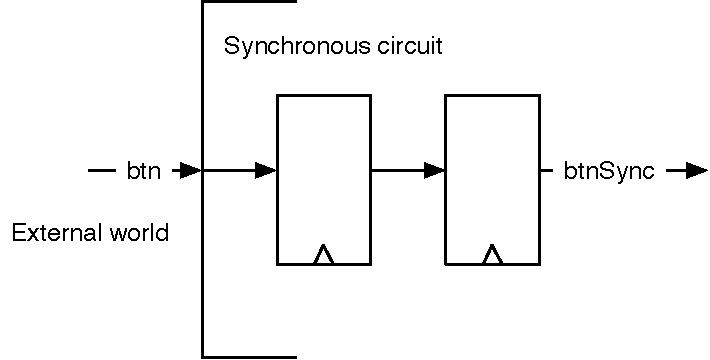
\includegraphics[scale=\scale]{../figures/synchronizer}
\end{figure}
\shortlist{../code/input_sync.txt}
\end{frame}

\begin{frame}[fragile]{Bouncing Buttons}
\begin{itemize}
\item Buttons and switches need some time to transition between on and off
\item May bounce between the two values
\item Without processing we detect more than one event
\item Solution is to filter out bouncing
\begin{itemize}
\item Can be done electrically
\item That is why you have the extra PCB with the buttons
\item But we can also do this digital
\end{itemize}
\item Assume  bouncing time $t_{bounce}$
\item Sample at a period $T > t_{bounce}$
\item Only use sampled signal
\end{itemize}
\end{frame}


\begin{frame}[fragile]{Sampling for Debouncing}
\begin{figure}
  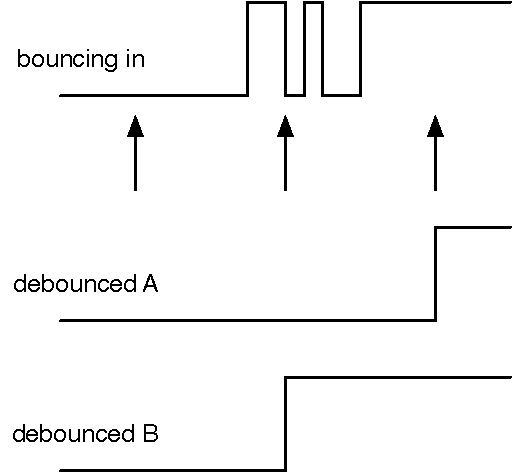
\includegraphics[scale=\scale]{../figures/debounce}
\end{figure}
\end{frame}


\begin{frame}[fragile]{Sampling for Debouncing}
\shortlist{../code/input_fac.txt}
\shortlist{../code/input_debounce.txt}
\begin{itemize}
\item We already know how to do this!
\item Just generate timing with a counter
\item We sample at 100 Hz (bouncing below 10 ms)
\end{itemize}
\end{frame}


\begin{frame}[fragile]{Noisy Input Signal}
\begin{itemize}
\item Sometimes input may be noisy
\item May contain spikes
\item Filtering with majority voting
\item Majority voting of the sampled input signal
\item However, this is seldom needed
\item Not for he buttons
\end{itemize}
\end{frame}


\begin{frame}[fragile]{Majority Voting}
\begin{figure}
  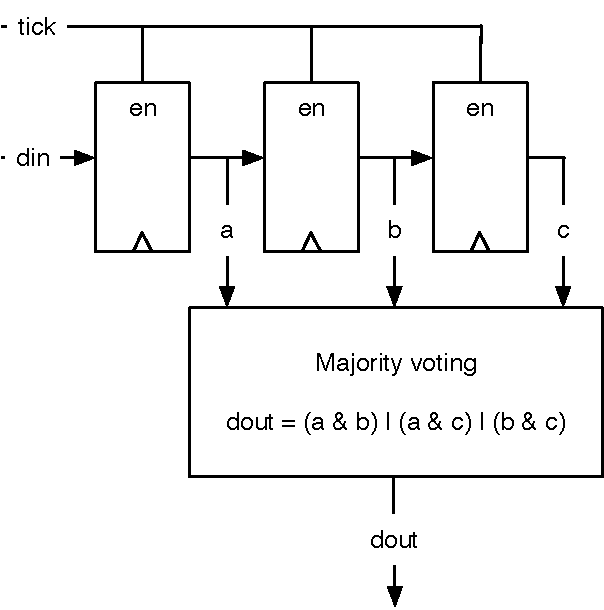
\includegraphics[scale=\scale]{../figures/majority}
\end{figure}
\end{frame}


\begin{frame}[fragile]{Majority Voting}
\shortlist{../code/input_majority.txt}
\end{frame}

\begin{frame}[fragile]{Detecting the Press Event}
\begin{itemize}
\item Edge detection
\item You have seen this before
\item Just to complete the input procssing
\end{itemize}
\shortlist{../code/input_usage.txt}
\end{frame}

\begin{frame}[fragile]{Combine Input Processing with Functions}
\begin{itemize}
\item Using small functions to abstract the processing
\item \href{https://github.com/schoeberl/chisel-book/blob/master/src/main/scala/Debounce.scala}{Debounce.scala}
\end{itemize}
\end{frame}

\begin{frame}[fragile]{Communicating State Machines}
\begin{itemize}
\item We did refactor a large FSM into smaller ones last week
\item FSMs \emph{communicate}
\item Simple communication is your input processing to FSM with datapath
\item More complex FSMs may exchange data with handshaking
\end{itemize}
\end{frame}

\begin{frame}[fragile]{Handshaking}
\begin{itemize}
\item Producer of data and consumer need to agree when data is transferred
\item Producer tells when data is available/valid with a \code{valid} signal
\item Consumer tells when it is ready toe receive data with a \code{ready} signal
\item When both are asserted the transfer takes place
\item Also called \emph{flow control}
\end{itemize}
\end{frame}

\begin{frame}[fragile]{Ready-Valid Interface}
\begin{figure}
  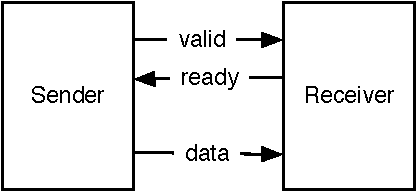
\includegraphics[scale=\scale]{../figures/readyvalid}
\end{figure}
\begin{itemize}
\item Ready-valid flow control
\end{itemize}
\end{frame}

\begin{frame}[fragile]{Ready-Valid Interface, Early Ready}
\begin{figure}
  \includegraphics[scale=1]{../figures/ready_valid1}
\end{figure}
\end{frame}

\begin{frame}[fragile]{Ready-Valid Interface, Late Ready}
\begin{figure}
  \includegraphics[scale=1]{../figures/ready_valid2}
\end{figure}
\end{frame}

\begin{frame}[fragile]{Single Cycle and Back-to-Back}
\begin{figure}
  \includegraphics[scale=1]{../figures/ready_valid3}
\end{figure}
\end{frame}

\begin{frame}[fragile]{Common Interface}
\begin{itemize}
\item So common interface that Chisel defines a \code{DecoupledIO}
\end{itemize}
\shortlist{../code/fifo_decoupled.txt}
\end{frame}

\begin{frame}[fragile]{First Summary and Break}
\begin{itemize}
\item Main topic of today done
\item Following is advanced material
\item A little bit of Scala
\item How to write hardware generators
\item Maybe extend your display to show decimal number
\item But first 10 minutes BREAK
\end{itemize}
\end{frame}


\begin{frame}[fragile]{Binary-Coded Decimal (BCD)}
\begin{itemize}
\item Your current display shows numbers in hexadecimal 
\begin{itemize}
\item $15_{10}$ is displayed as $0F_{16}$
\item Which is in binary: 00001111
\item We would like to see it as a `1' followed by a `5'
\item Which is in binary: 0001 0101
\end{itemize}
\item Convert from binary to binary-coded decimal (BCD)
\begin{itemize}
\item But only for the display
\item Computing in BCD is hard
\end{itemize}
\end{itemize}
\end{frame}

\begin{frame}[fragile]{Binary to BCD Conversion Table}
\begin{chisel}
  val bincode = io.sw(7,0)
  val bcd = WireDefault(bincode)

  switch(bincode) {
    is(0.U) { bcd := "b0000_0000".U }
    is(1.U) { bcd := "b0000_0001".U }
    is(2.U) { bcd := "b0000_0010".U }
    // ... some more
    is(9.U) { bcd := "b0000_1001".U }
    is(10.U) { bcd := "b0001_0000".U }
    is(11.U) { bcd := "b0001_0001".U }
    is(12.U) { bcd := "b0001_0010".U }
    // ... and many more entries
  }

  dispMux.io.price := bcd
\end{chisel}
\end{frame}

\begin{frame}[fragile]{Binary-Coded Decimal (BCD)}
\begin{itemize}
\item Conversion is a table (= function)
\item Combinational logic
\item We \emph{could} do the table manually
\begin{itemize}
\item But it is large
\item The table has 100 entries to convert 0 to 99 to BCD
\end{itemize}
\item Let's write a program for this
\item We will write our first \emph{hardware generator}
\item First we need a little bit of Scala
\end{itemize}
\end{frame}



\begin{frame}[fragile]{Chisel and Scala}
\begin{itemize}
\item Chisel is a library written in Scala
\begin{itemize}
\item Import the library with \code{import chisel3.\_}
\end{itemize}
\item Chisel code is Scala code
\item When it is run is \emph{generates} hardware
\begin{itemize}
\item Verilog for synthesize
\item Scala netlist for simulation (testing)
\end{itemize}
\item Chisel is an embedded domain specific language
\item Two languages in one can be a little bit confusing
\end{itemize}
\end{frame}

\begin{frame}[fragile]{Scala}
\begin{itemize}
\item Is object oriented
\item Is functional
\item Strongly typed with very good type inference
\item Runs on the Java virtual machine
\item Can call Java libraries
\item Consider it as Java++
\begin{itemize}
\item Can almost be written like Java
\item With a more lightweight syntax
% \item Scala for Java Refugees is a nice tutorial (but link is dead)
% \item \url{http://www.codecommit.com/blog/scala/roundup-scala-for-java-refugees}
\end{itemize}
\end{itemize}
\end{frame}

\begin{frame}[fragile]{Scala Hello World}
\shortlist{../src/main/scala/HelloScala.scala}
\begin{itemize}
\item Compile with \code{scalac} and run with \code{scala}
\item You can even use Scala as a scripting language
\item Or run with \code{sbt run}
\item Show both
\end{itemize}
\end{frame}

\begin{frame}[fragile]{Scala Values and Variables}
\begin{itemize}
\item Chisel has two type of variables: \code{val}s and \code{var}s
\item A \code{val} cannot be reassigned, it is a constant
\item We use a \code{val} to name a hardware component in Chisel
\end{itemize}
\shortlist{../code/scala_val.txt}
\begin{itemize}
\item Types are usually inferred
\item But can be explicitly stated as follows
\end{itemize}
\shortlist{../code/scala_int_type.txt}
\end{frame}

\begin{frame}[fragile]{Scala Variables}
\begin{itemize}
\item A \code{var} can be reassigned, it is like a classic variable
\item We use a \code{var} to write a hardware generator in Chisel
\end{itemize}
\shortlist{../code/scala_var.txt}
\end{frame}

\begin{frame}[fragile]{Simple Loops}
\shortlist{../code/scala_loop.txt}
\begin{itemize}
\item We use a loop to generate hardware components
\end{itemize}
\end{frame}

\begin{frame}[fragile]{Scala \code{for} Loop for Circuit Generation}
\shortlist{../code/scala_loop_gen.txt}
\begin{itemize}
\item \code{for} is Scala
\item This loop generates several connections
\item The connections are parallel hardware
\item This is a shit register
\end{itemize}
\end{frame}

\begin{frame}[fragile]{Conditions}
\shortlist{../code/scala_condition.txt}
\begin{itemize}
\item Executed at runtime, when the circuit is created
\item This is \emph{not} a mlutplexer
\end{itemize}
\end{frame}

\begin{frame}[fragile]{Scala Arrays and Lists}
\begin{chisel}
// An integer array with 10 elements
val numbers = new Array[Integer](10)
for (i <- 0 until numbers.length) {
  numbers(i) = i*10
}
println(numbers(9))


// List of integers
val list = List(1, 2, 3)
println(list)
// Different form of list construction
val listenum = 'a' :: 'b' :: 'c' :: Nil
println(listenum)
\end{chisel}
\end{frame}


\begin{frame}[fragile]{Scala Classes}
\begin{chisel}
// A simple class
class Example {
  // A field, initialized in the constructor
  var n = 0
  
  // A setter method
  def set(v: Integer) = {
    n = v
  }
  
  // Another method
  def print() = {
    println(n)
  }
}
\end{chisel}
\end{frame}

\begin{frame}[fragile]{Scala (Singleton) Object}
\begin{chisel}
object Example {}
\end{chisel}
\begin{itemize}
\item For \emph{static} fields and methods
\begin{itemize}
\item Scala has no static fields or methods like Java
\end{itemize}
\item Needed for \code{main}
\item Useful for helper functions
\end{itemize}
\end{frame}

\begin{frame}[fragile]{Singleton Object for the \code{main}}
\begin{chisel}
// A singleton object
object Example {
  
  // The start of a Scala program
  def main(args: Array[String]): Unit = {
    
    val e = new Example()
    e.print()
    e.set(42)
    e.print()
  }
}
\end{chisel}
\begin{itemize}
\item Compile and run it with sbt (or within Eclipse/IntelliJ):
\end{itemize}
\begin{chisel}
sbt "runMain Example"
\end{chisel}
\end{frame}







\begin{frame}[fragile]{Conditional Circuit Generation}
\begin{chisel}
class Base extends Module { val io = new Bundle() }
class VariantA extends Base { }
class VariantB extends Base { }

val m = if (useA) Module(new VariantA())
        else Module(new VariantB())
\end{chisel}
\begin{itemize}
\item \code{if} and \code{else} is Scala
\item \code{if} is an expression that returns a value
\begin{itemize}
\item Like ``\code{cond ? a : b;}'' in C and Java
\end{itemize}
\item This is not a hardware multiplexer
\item Decides which module to generate
\item Could even read an XML file for the configuration
\end{itemize}
\end{frame}


\begin{frame}[fragile]{A Table with a Chisel \code{Vec}}
\begin{itemize}
\item A Chisel \code{Vec} is a collection of signals or registers
\item Similar to an Array in other languages
\item \code{Vec} in a \code{Wire} is a combinational table
\item \code{Vec} in a \code{Reg} is a collection of registers
\item Create with number of elements and hardware type
\end{itemize}
\shortlist{../code/vec.txt}
\end{frame}

\begin{frame}[fragile]{A Combinational \code{Vec}}
\begin{itemize}
\item A combinational \code{Vec} is basically a multiplexer
\item Input signal/wire connected with a constant index
\item Output select with a Chisel \code{UInt} signal
\end{itemize}
\shortlist{../code/vec_access.txt}
\begin{itemize}
\item Also convenient to represent a larger table
\begin{itemize}
\item Instead of a \code{switch} table
\item Input can be \emph{generated} with Scala code
\end{itemize}
\end{itemize}
\end{frame}

\begin{frame}[fragile]{Binary to BCD Convertion}
\shortlist{../code/bcd_table.txt}
\end{frame}



\begin{frame}[fragile]{Summary}
\begin{itemize}
\item External inputs need processing
\item Minimum is a input synchronizer
\item Communicating circuits/FSMs need handshaking
\item Reard-valid interface
\item Scala can be used to write circuit \emph{generators}
\item We explored generation of a binary to BCD conversion table
\end{itemize}
\end{frame}



\end{document}

%\begin{frame}[fragile]{xxx}
%\begin{itemize}
%\item yyy
%\end{itemize}
%\end{frame}
